\documentclass[a4paper, 12pt]{article}
\usepackage[hmargin=1.25in,vmargin=1in]{geometry}

\usepackage{xeCJK}

%% Font
\CJKfontspec{Noto Serif CJK TC} % 思源宋體

\usepackage{parskip}
\setlength{\parindent}{2em} % 縮排兩個字
\usepackage{indentfirst}
 
\usepackage{listings} % Maybe for code block
\usepackage{underscore}

% If you don't like separate files, use this:
% \usepackage{filecontents}
% \begin{filecontents}{references.bib}
% @online{csie_restaurant,
%   author = "{guyleaf, asd3013593, RonToSucceed, a58176197, Andersonabc, orz123789}",
%   title = "CSIE restaurant 孜宮庭園-北科大校園外送平台",
%   url  = "https://github.com/guyleaf/csie_restaurant",
% }
% @online{aws_arch_diagram,
%   author = "Amazon Web Services",
%   title = "What Is Architecture Diagramming?",
%   url  = "https://aws.amazon.com/what-is/architecture-diagramming",
% }
% \end{filecontents}

\usepackage[autocite=superscript]{biblatex}
\addbibresource{references.bib}

\usepackage{graphicx}
\graphicspath{ {./images/} }

\usepackage{hyperref}
\hypersetup{
    colorlinks=true,
    linkcolor=black,
    filecolor=magenta,      
    urlcolor=cyan,
    pdftitle={Overleaf Example},
    pdfpagemode=FullScreen,
} % Copy from https://www.overleaf.com/learn/latex/Hyperlinks

% Custom varibles
\def\myProjectName{專案名稱(Project Name)}
\def\myVersion{1.0}

% Font Size
\newcommand\TwentyTitle{\fontsize{20pt}{24pt}\selectfont}
\newcommand\EighteenTitle{\fontsize{18pt}{20pt}\selectfont}
\newcommand\SixteenTitle{\fontsize{16pt}{18pt}\selectfont}
\newcommand\SectionFont{\fontsize{14pt}{16pt}\selectfont}
\newcommand\NormalFont{\fontsize{12pt}{16pt}\selectfont}

\usepackage{titlesec}
\titleformat*{\section}{\center\SectionFont\bfseries}
\titleformat*{\subsection}{\NormalFont\bfseries}
\titleformat*{\subsubsection}{\NormalFont}

\renewcommand{\arraystretch}{1.2} % table row height

%----------------------------------------------------------

\begin{document}

%titlepage
\thispagestyle{empty}
\begin{center}
    {\TwentyTitle \myProjectName \par}
    \vspace{6cm}
    {\TwentyTitle 系統需求規格書 \par}
    {\EighteenTitle Software Requirements Specification (SRS) \par}
    {\SixteenTitle Version: \myVersion \par}
    \vspace{4cm}
    {\SixteenTitle
    \begin{tabular}{ccc}
      姓名 & 學號 & E-mail \\[0.2em]
      劉建宏 & 000000000 & t000000000@ntut.org.tw \\
      劉建宏 & 000000000 & t000000000@ntut.org.tw \\
      劉建宏 & 000000000 & t000000000@ntut.org.tw \\
      劉建宏 & 000000000 & t000000000@ntut.org.tw \\
      劉建宏 & 000000000 & t000000000@ntut.org.tw \\
      劉建宏 & 000000000 & t000000000@ntut.org.tw \\
    \end{tabular}
    \par}
    \vspace{2cm}
    {\SixteenTitle Department of Computer Science \& Information Engineering National Taipei University of Technology \par}
    \vspace{16pt}
    {\SixteenTitle 10/11/2023 \par}
\end{center}
\clearpage

\renewcommand{\contentsname}{目錄 (Table of Contents)}
\tableofcontents
\newpage

%---------------------------------------------

% \section*{Revision History}

% \begin{center}
%     \begin{tabular}{|c|c|c|c|}
%         \hline
% 	    Name & Date & Reason For Changes & Version\\
%         \hline
% 	    21 & 22 & 23 & 24\\
%         \hline
% 	    31 & 32 & 33 & 34\\
%         \hline
%     \end{tabular}
% \end{center}

% \newpage
%----------------------------------------------

\section{簡介 (Introduction)}

\subsection{目的 (Purpose)}

藉由本學期修習的資料庫系統課程,為了更加理解資料庫的運行及流程的設計,並且將過往學習到的網頁程式設計、網際網路技術與應用和各項程式語言的基礎學以致用,透過分工合作完成使用資料庫的系統,因此我們決定開發一個完整的美食商場系統「孜宮庭園\autocite{csie_restaurant}」,此系統能讓使用者可以在網路上進行搜索、瀏覽、預約餐點和便捷的外送服務,藉由畫面精緻且簡易上手的介面,讓大家擁有賓至如歸的服務及美食體驗。

\noindent 本系統主要目標為:
\begin{enumerate}
  \item 目的一
  \item 目的二
  \item 目的二
  \item 目的二
  \item 目的二
\end{enumerate}


\subsection{系統名稱 (Identification)}

\noindent 本專案範圍包含建置下面主系統與各項子系統,主系統為:

\begin{itemize}
  \item 外星人培根貓龍系統 (Alien Bacon Cat Dragons System, ABCDS)
\end{itemize}

\noindent 子系統為:

\begin{itemize}
  \item 外星人培根貓龍子系統 (Alien Bacon Cat Dragons Subsystem, ABCDS)
  \item 外星人培根貓龍子系統 (Alien Bacon Cat Dragons Subsystem, ABCDS)
  \item 外星人培根貓龍子系統 (Alien Bacon Cat Dragons Subsystem, ABCDS)
  \item 外星人培根貓龍子系統 (Alien Bacon Cat Dragons Subsystem, ABCDS)
\end{itemize}


\subsection{概觀 (Overview)}

藉由本學期修習的資料庫系統課程,為了更加理解資料庫的運行及流程的設計,並且將過往學習到的網頁程式設計、網際網路技術與應用和各項程式語言的基礎學以致用,透過分工合作完成使用資料庫的系統,因此我們決定開發一個完整的美食商場系統「孜宮庭園」,此系統能讓使用者可以在網路上進行搜索、瀏覽、預約餐點和便捷的外送服務,藉由畫面精緻且簡易上手的介面,讓大家擁有賓至如歸的服務及美食體驗。


\subsection{符號描述 (Notation Description) (if any)}

\newcommand{\notationDescTableCol}{ | p{6.5em} | p{32em} |}

\noindent \begin{tabular}{\notationDescTableCol}
  \hline
  Notation & Description \\
  \hline
  ABCDS 1.0.0 & Alien Bacon Cat Dragons System will be labeled with the number 1.0.0 \\
  ABCDS 1.1.n & Alien Bacon Cat Dragons Subsystem will be labeled with the number 1.1.n \\
  ABCDS 1.1.n & Alien Bacon Cat Dragons Subsystem will be labeled with the number 1.1.n \\
  ABCDS 1.1.n & Alien Bacon Cat Dragons Subsystem will be labeled with the number 1.1.n \\
  ABCDS 1.1.n & Alien Bacon Cat Dragons Subsystem will be labeled with the number 1.1.n \\
  \hline
\end{tabular} \par

\noindent \begin{tabular}{\notationDescTableCol}
  \hline
  Notation & Description \\
  \hline
  ABCDS-I-nnn & ABCDS 介面需求(Interface Requirements) \\
  ABCDS-F-nnn & ABCDS 功能性需求(Functional Requirements) \\
  ABCDS-D-nnn & ABCDS 資料需求(Data Requirements) \\
  ABCDS-N-nnn & ABCDS 非功能性需求(Non-Functional Requirements) \\
  ABCDS-O-nnn & ABCDS 其他需求(Other Requirements) \\
  ABCDS-B-nnn & ABCDS 商業規則或約束 (Business Rules or Constraints) \\
  \hline
\end{tabular} \par

\newpage

\section{系統 (System)}
\subsection{系統描述 (System Description)}
\subsubsection{系統架構圖 (System Architecture Diagram) }
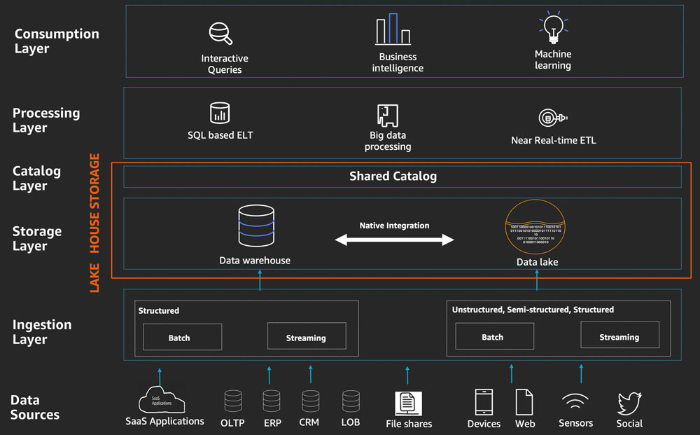
\includegraphics[width=30em]{arch-digram.png}
\cite{aws_arch_diagram}

\subsection{操作概念 (Operational Concepts or User Stories)}
\subsection{功能性需求 (Functional Requirements)}
\subsection{資料需求 (Data Requirements)}
\subsection{非功能性需求 (Non-Functional Requirements)}
\subsubsection{效能需求 (Performance Requirements)}
\subsubsection{資安需求 (Security Requirements) (if any)}
\subsection{介面需求 (Interface Requirements)}
\subsubsection{使用者介面需求 (User Interfaces Requirements)}
\subsubsection{外部介面需求 (External Interface Requirements) (if any)}
\subsubsection{內部介面需求 (Internal Interface Requirements) (if any)}
\subsection{其他需求 (Other Requirements)}
\subsubsection{環境需求 (Environmental Requirement)}
\subsubsection{安裝需求 (Installation Requirement)}
\subsubsection{測試需求 (Test Requirements) (if any)}
\subsection{商業規則與限制 (Business Rules and Integrity Constrains)}
\newpage

\section{Glossary}
\newpage

\section{References}
\printbibliography[heading=none]
\newpage

\section{Appendix}
\newpage

\end{document}
